\chapter{Core reference}
\section{\module{pyDCPU} --- 
        \textbf{Py}thon \textbf{D}ata \textbf{C}ollect and \textbf{P}rocess \textbf{U}nit}

\declaremodule[pyDCPU]{}{pyDCPU}       

\moduleauthor{Hannes Matuschek}{hmatuschek@gmx.net}


\modulesynopsis{This is the reference for the core-library of PPLT System.}

The \module{pyDCPU} module provides all needed core methods and functions, to
get a PPLT system running. The library implements the basic features like 
loading modules (Master/Exporter), managing the symbol-tree 
(create/move/delete/chmod/chown/chgrp/...) and managing the user
data base. Usually the \module{pyDCPU} library provides all the functionality
of the PPLT system. 

%\subsection{Concept} 
The core of the PPLT system have to provide all the functionality to access devices
by master-slave based communication channels and handle the values read back into
a central place. Also these values should be served to other applications, independent
from the interface the application use. So the core is divided into three major parts.

\begin{figure}[ht]
    \centering
    \label{cDCPU}
    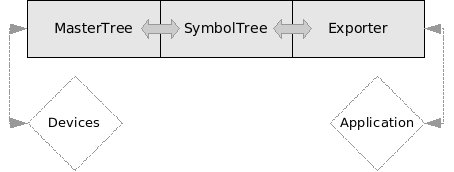
\includegraphics[scale=1]{cDCPU.png}
    \caption{Parts of the core.}
\end{figure}

The first called \textit{Master-Tree}. This provide the access to the devices. The 
second part called \textit{Symbol-Tree} holds all values in a filesystem like 
hierarchy. The last part, the \textit{Exporters}, serves the symbol-tree to other
applications like a visualization. This concept is very common for this kind of 
problems. 

\subsection{The Master-Tree}
To access the devices a master-slave based communication is often used. This are 
for example the common BUSes and also TCP/IP like networks. All these protocols
have one basic concept; they are separable into layers. Each layer encapsulate 
an element of the communication.  For TCP/IP this is the famous OSI reference 
model. So it is useful to implement each layer of the communication channel
into separate modules to have the facility to reuse some of the modules. By
this you only need to implement these layers of the communication, that aren't
implemented yet to access a new device. For example if you want to access
a unsupported device that uses an already implemented BUS you'll need only
to write a module that implements the command messages for this device.

A common way to separate the communication is to differ between the used
interface, transport-protocol, and command-messages. The interface provides
the access to the BUS hardware, for example the serial-interface. The 
transport-protocol or BUS protocol uses the interface and generate valid 
messages that reaches the device. The module that generates the 
command-messages uses the transport-protocol to send the messages to the
device and to wait for an answer.  

\begin{figure}[ht]
    \centering
    \label{fig:cMasterTree}
    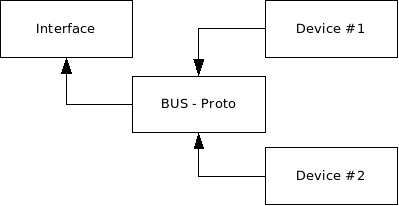
\includegraphics[scale=1]{cMasterTree.png}
    \caption{Scheme of Master-Tree concept with shared interface and BUS modules.}
\end{figure}

An common scenario would be: You want to get a value from a device. So
you read from the module-object that implements the command messages.
This module will send a command-message over the BUS (protocol and interface)
to the device. Then the module will waits for an answer of the device
by reading from the BUS (over protocol and interface module). The
answer will be dispatched and you'll get the value.

If one module read from or writes to an other module the modules
will be locked and no other module can access these modules. By this way 
BUS collisions are avoided. And on the other hand if you want to access
two devices that are connected to the same BUS, you'll setup a 
Master-Tree where the device-modules \#1 and \#2 share the modules for the 
interface and BUS. Now you see why the Master-Tree is called a tree (forest 
would be better). The root of each tree is the interface and the leafs are 
the devices.

To get the all module work together a clear API between the modules have
to be defined, so that you don't have to adjust the modules to work together
with other/new modules. 

\subsection{The Symbol-Tree}
Once the access to the devices is set up, you need to care about what values 
should be served. Each device will be able to provide a lot of different values
and a user or application don't know how to get a specific value. So you'll 
need a abstraction of the set of values. On the other hand, if you want to 
serve a lot of values you want to group the values by there sense and not by the
devices they are come from. So the idea of a \textit{filesystem} raises that holds 
the values in \textit{symbols} grouped in \textit{folders}, independent of the 
device the value was read from. At this point it will be useful to control
who have access to a specific value (symbol). 

A symbol is usually directly connected to a device-module. That means, if you 
want to get the value of the symbol, the symbol asks the device-module to read
the value from the device. But it is also possible to connect a symbol to a
module that implements a BUS protocol. By this you'll be able to tunnel the 
BUS to an other application of the Internet. If you read out of such a symbol
you'll read directly from BUS and if you write into the symbol you'll write 
into the BUS. But be careful with exporting the BUS to other networks, you
can't control what messages are sent over the BUS!


\subsection{Exporter}
The last part of the core exports the symbol-tree, or maybe a part of it, to
other applications. So the PPLT system is able to support a wide range of 
applications, independent of the protocol or interface the application
will use. Also the exporter are implemented as modules. But in this case
the communication with the exporters are not separated into separate modules.
Each exporter is run into its own thread. So it is possible to handle
different applications with several instances at the same time. 


\section{Exceptions}
In this section I will list and describe all exceptions that may be raised by 
the \module{pyDCPU}-\class{Core}. 

\begin{excclassdesc}{Error}{\optional{\var{ErrMsg}}}
This is the base exception-class. All exceptions raised by the core will be
this class or one derived from this. So you can catch all exceptions raised
by the core by:
\verbatiminput{exception01.py}
You can (optional) set an error message to the exception by the argument
\var{ErrMsg}.
\end{excclassdesc}

\begin{excclassdesc}{ItemBusy}{\optional{\var{ErrMsg}}}
This exception will be raised if an item is in busy in any case. For example,
if you want to unload an core-module until it is used by symbols or other 
modules, if you want to read/write from/to an symbol or module, that is locked
by an other thread, and so on. 
This exception will be raise if an item is in use. 
\end{excclassdesc}

\begin{excclassdesc}{ItemNotFound}{\optional{\var{ErrMsg}}}
This exception will be raised if an item (Module, Symbol Folder, ...) can not
be found. Like the exception \exception{ItemBusy} this one is not bound to an
specific case and can be raised by nearly any method of \class{core}.
\end{excclassdesc}

\begin{excclassdesc}{AccessDenied}{\optional{\var{ErrMsg}}}
This exception will be raised if you're have not the right to access a item.
This exception is also like \exception{ItemBusy} not bound to an specific 
context! But it will be raised mostly in the context of the symbol-tree. 
Therefor you should care for it if you write an server-module (called Exporter
here). 
\end{excclassdesc}

\begin{excclassdesc}{ModuleError}{\optional{\var{ErrMsg}}}
This is the base exception for all errors bound to the modules, like an 
setup-error or if a module can't be loaded. 
\end{excclassdesc}

\begin{excclassdesc}{BadModule}{\optional{\var{ErrMsg}}}
This exception is derived from \exception{ModuleError}. It will be raised if
a module has a wrong API or no meta-file. Even if you try to load a \emph{bad}
module. 
\end{excclassdesc}

\begin{excclassdesc}{ModuleRequirement}{\optional{\var{ErrMsg}}}
This exception (derived from \exception{ModuleError}) will be raised if a 
requirement of the module is not satisfied. Meaning you have the wrong 
python-version or a needed package is not installed. 
\end{excclassdesc}

\begin{excclassdesc}{ModuleSetup}{\optional{\var{ErrMsg}}}
This exception (derived from \exception{ModuleError}) will be raised if the
setup of the module fails. This exception will be raised normally by the 
module and may contain any information about the reason of failure.
\end{excclassdesc}

\begin{excclassdesc}{SymbolError}{\optional{\var{ErrMsg}}}
This is the base-exception for all symbol-related-stuff. \notice{The case "a 
Symbol is not found" is covert by the \exception{ItemNotFound} exception and 
in the case that you don't have the right to access a symbol a 
\exception{AccessDenied} exception will be raised.}
\end{excclassdesc}


\section{Class description}
In this section I will describe the core-class. This class holds all methods
you'll need. All work will be done by calling methods of an instance of this
class.

\begin{classdesc}{Core}{\optional{ModulePath, \optional{UserDBFile, \optional{LogLevel, \optional{LogFile, \optional{SysLog}}}}}}
This is the all-in-one class of the \module{pyDCPU}. All work like loading 
modules will be done by calling methods of this class. 

Creates a new core-instance. The optional argument \var{ModulePath} specifies
the base-path to the core-modules. If missed, the default path 
\texttt{sys.exec\_path+"/PPLT"} will be used. 

The argument \var{UserDBFile} specifies the filename of the used database to 
be loaded. If missed the default file 
(\texttt{sys.exec\_path+"/PPLT/UserDB.xml"}) will be used.


The argument \var{LogLevel} specify the log-level and so the verbosity of the 
core. This should be one of (\code{'off'}, \code{'fatal'}, \code{'error'}, 
\code{'info'} or \code{'debug'}). Note that \code{'off'} switches the logging
off and \code{'debug'} will produce a lot of messages. 

In normal case all logging massages were printed on the screen (send to 
stderr) but with the arguments \var{LogFile} and \var{SysLog} you can 
manipulates this behavior. If the argument \var{LogFile} is given, this file 
will be used to log all messages to. Note, that if \var{LogFile} specified no 
messages are shown on stderr. If \var{SysLog} is \code{True} all log messages 
will be send to the local syslog-daemon. Note this argument overrides the 
setting of \var{LogFile} and also no messages were send to stderr.

While instancing this class a \exception{Error}-exception may be raised. So the 
best way to instance the Core-class may:
\verbatiminput{core01.py}
\end{classdesc}

\section{Methods of \class{Core}}
\label{core-objects}
In the following section I will describe all methods of the \class{Core} 
class. 


\subsection{Mastertree methods}
\begin{methoddesc}[Core]{MasterTreeAdd}{ParentID, ModName, Address, Parameter}
This method loads an instance of a core-module and adds it to the master-tree. 
The method returns the ID of the loaded module. This ID is unique but if you 
load the same module with the same parameters, address and at the same parent, 
the ID of the ID of the already loaded module will be returned.

The argument \var{ParentID} specifies the parent-module (ID), the new loaded 
module will be attached to. If you set \var{ParentID} to \code{None} the 
module will be loaded as a root\footnote{A root-module has no parent module.}. 

The argument \var{ModName} specifies the full qualified name of the module. 
All modules are organized in classes and subclasses. A full qualified name 
would be a module-name with all classes and subclasses divided by single dots. 
For example: \code{Master.Interface.UniSerial} or \code{Master.Device.S7-200}.

The argument \var{Address} specifies the address used to connect the parent 
module. If there is no parent, meaning \var{ParentID} is \code{None}, or there
is no need to addressing the parent-module, the argument \var{Address} should 
be \code{None}.

The argument \var{Parameter} specifies the parameter used to load (and setup) 
the module. This argument should be a dict.  The keywords are the parameters 
names (all strings) and the values are the values of the singe parameter.  
\notice{All parameter values are strings!} If the module needs no parameters, 
please set \var{Parameter} to \code{None} or to an empty dict \code{\{\}}.

This method raises an exception derived from base-exception \exception{Error} 
on error. So an \exception{ItemNotFound}-exception will be raised if no 
matching object for \var{ParentID} or if no module named \var{ModName} can be 
found. A \exception{ModuleSetup} will be raised if the setup of the module
fails. 

An example for loading all modules to access an Siemens SIEMATIC S7-200:
\verbatiminput{core02.py}
\end{methoddesc}


\begin{methoddesc}[Core]{MasterTreeDel}{ObjectID}
This method removes an (module-)object from the master-tree and destroy it. 
\note{The object mast have no children, meaning no other objects  
are connected to this object.}

The argument \var{ObjectID} specifies the object you want to remove. This 
object ID is the ID you got by the \function{MasterTreeAdd()} method-call.

If no loaded module can be found with id \var{ObjectID}, a 
\exception{ItemBusy}-exception will be raised! May an other
exception, derived from the \exception{Error}-exception, will be
raised if the unload fails.
\end{methoddesc}


\begin{methoddesc}[Core]{MasterTreeList}{ParentID}
This method will list the IDs of all children of the given module-instance. The argument \var{ParentID} specifies the 
ID of the module-instance, that children will be listed. If \code{None} is given, all \emph{root} 
module-instances \footnote{Root module-instances are all modules, that have no children.}
were listed. This method will raise an \exception{ItemNotFound} if no object can be found for
\var{ParentID}.
\end{methoddesc}


\subsection{Symboltree methods}
\begin{methoddesc}[Core]{SymbolTreeCheckPath}{Path}
This method checks if the given \var{Path} exists. This method returns  \code{True} if the given path is a folder or symbol
and \code{False} otherwise.
\end{methoddesc}


\begin{methoddesc}[Core]{SymbolTreeCreateFolder}{Path}
This method creates a folder. 

The argument \var{Path} specifies the full path to the folder, that will be created. \note{The path should have the 
standard Linux format like: \code{'/path/to/new\_folder'}.}

This method will raise an exception derived from the \exception{Error}-exception-class on error. 
\end{methoddesc}


\begin{methoddesc}[Core]{SymbolTreeCreateSymbol}{Path, ObjectID, \optional{Address}, \optional{Timeout}}
This method will create a new symbol in the symbol-tree and connect it to the 
given Object.

The argument \var{Path} specifies the full path to the new symbol. This path 
should be in the standard Linux format like \code{'/path/to/new\_symbol'}.

The argument \var{ObjectID} specifies the object, the symbol will be connected
to. This is the ID you've got back from a \function{MasterTreeAdd} call. You can 
connect a symbol to any object, but you'll not get always useful values back 
from this object. You can also connect the symbol to an object, that doesn't provide
any values, for example to a object of the \code{UniSerial} module to tunnel the
serial interface to an external application by the symbol-tree.

The optional argument \var{Address} specifies the address to be used to connect
to the object. To find out what addresses are provided by a specific module,
please look at the \textit{Core Modules Reference}. Of the address is omitted,
no address will be used to connect to the object. In the most cases this means
to connect to the data chanel of the module. 

The optional argument \var{Timeout} specifies the caching time for the symbol in
seconds. The default value is 0.5s.
For this time the last read value is returned instead of reread the value each 
time. By this it is possible to reduce the traffic on BUS if may clients access 
the symbols.
\end{methoddesc}


\begin{methoddesc}[Core]{SymbolTreeDeleteFolder}{Path}
This method will remove the given folder. This folder should be empty before removing it.

The argument \var{Path} specifies the path of the folder that will be removed. 

This method will raise an \exception{ItemBusy} exception if the folder you 
want to delete is not empty.
\end{methoddesc}


\begin{methoddesc}[Core]{SymbolTreeDeleteSymbol}{Path}
This method will remove a symbol from the symbol-tree. 

The argument \var{Path} specifies the full path to the symbol, that will be removed.
This path should be in the standard Linux format like: \code{'/path/to/symbol'}.
\end{methoddesc}


\begin{methoddesc}[Core]{SymbolTreeListFolder}{Path}
This method list all folders in the folder pointed by \var{Path}.

The argument \var{Path} specifies the full path to the folder, that sub-folders
will be listed. 
\note{If you want to list all folders at the 
root-folder, you should use \code{'/'} as path.}

The method returns a list of subfolders or an empty list if the folder has no sub-folders.
\end{methoddesc}


\begin{methoddesc}[Core]{SymbolTreeListSymbols}{Path}
This method will list all symbols in the folder pointed by \var{Path}.

The argument \var{Path} specifies the full path to the folder, that symbols
will be listed. 

\note{If you want to list all symbols at the 
root-folder, you should set \var{Path} to \code{'/'}.}

The method will return a list of strings or an empty list if there are no 
symbols in the folder.
\end{methoddesc}


\begin{methoddesc}[Core]{SymbolTreeGetAccess}{Path}
This method will return the owner, group and access-rights of the given folder or symbol.

The argument \var{Path} specifies the path of the folder or symbol.

This method will raise an \exception{ItemNotFound} if the given \var{Path} 
doesn't exists.
\end{methoddesc}


\begin{methoddesc}[Core]{SymbolTreeSetAccess}{Path, Owner, Group, Modus}
This method will set the owner, group and access-rights of the given symbol or folder.

The argument \var{Path} specifies the full path of the symbol or folder.

The argument \var{Owner} specifies the owner of the symbol or folder, the 
argument \var{Group} specifies the group the symbol/folder will belong to.
At least the argument \var{Modus} specifies the access-rights of the
symbol/folder.

This method will raise an exception derived from \exception{Error} base-exception on error.
\end{methoddesc}


\begin{methoddesc}[Core]{SymbolTreeGetValue}{Path}
This method will return the value of the symbol pointed by \var{Path}.

The argument \var{Path} specifies the full path to the symbol. 

The method will return the value(s) of the symbol or \code{None} on error.
\end{methoddesc}


\begin{methoddesc}[Core]{SymbolTreeSetValue}{Path, Value}
This method will set the value of the symbol pointed by \var{Path} to \var{Value}.

The argument \var{Path} specifies the full path to the symbol, that value will be set.

The argument \var{Value} specifies the value(s) the symbol will be set to.

This method will raise an exception derived from \exception{Error}-exception. 
\notice{Please contatct the author if you notice the raise of an other (not 
\exception{Error} based) exception. This is regulary an error in a module.}
\end{methoddesc}


\begin{methoddesc}[Core]{SymbolTreeRead}{Path, \optional{Length}}
This method will read (\var{Length}) bytes from symbol given by \var{Path}. 
The argument \var{Length} is optional, and means (if missed) that you want
to read a sequence out of the symbol. If the symbol is connected to a stream,
you will get only one by back from stream. Otherwise you'll read \var{Length} 
bytes from stream or sequence symbol. This method will may raise an exception 
derived form \exception{Error} base-exception on error.
\end{methoddesc}


\begin{methoddesc}[Core]{SymbolTreeWrite}{Path, Data}
This method will write the data given by \var{Data} into the
symbol given by \var{Path}. This method works like the method
\method{SymbolTreeSetValue}.
\end{methoddesc}


\subsection{Exporter methods}
\begin{methoddesc}[Core]{ExporterAdd}{ExportModule, Parameters, DefaultUser, \optional{Root='/'}}
This method will load and setup a exporter module. A exporter is something like
you may call a server.To successfully setup the module, some module specific 
parameters are needed. Also you can set a default user which rights will be 
used, if the exporter doesn't support any kind of authentication. Optional you can set 
a server-root. The server root should be a folder in the symbol tree. If a exporter 
is loaded with the \var{Root} option, only the symbols under the server-root 
and the sub-folders of this root are exported by the server.

The argument \var{ExportModule} specifies the full qualified name of the 
exporter-module. A full qualified name contains all classes and subclasses of 
the exporter. For example: \code{'Export.JVisu'}. 

The argument Parameters specifies the parameters, the export-module needs to be
successfully set up. The parameters are given as a dict. The keys of the dict
are the names of the parameters and the values are the values of the 
parameters. If the export-module needs no parameters, please set 
\var{Parameters} to \code{None} or to an empty dict.

The argument \var{DefualtUser} specifies the name of the user, the server will 
get his rights from. This can be used to control the rights of a exporter,
that doesn't know any authentication.

The optional argument \var{Root} specifies the server-root for this exporter. 
If you miss this argument or set it to \code{'/'}, the whole symbol-tree
will be exported by this server. Otherwise only the symbols and sub-folders of
the given folder were be exported.

This method will return the ID of the new loaded exporter. On error an 
exception derived from the \exception{Error} exception will be raised.
\end{methoddesc}


\begin{methoddesc}[Core]{ExporterList}{}
This method lists the IDs of all loaded exports (servers). The method returns
a list of strings containing the IDs you got by the \function{ExporterAdd()}
method-call. 
\end{methoddesc}


\begin{methoddesc}[Core]{ExporterDel}{ObjectID}
This method will stop and remove the exporter pointed by the given ID. 

The argument \var{ObjectID} specifies the exporter, that should be removed.
This is the ID you got by the \function{ExporterAdd} method-call.

\end{methoddesc}
